\begin{tikzpicture}
  \draw [thick,->,green] 
    (0,0) -- ++(3,0) 
      node [pos=0.5,below,black,align=center] {$k_L \sin \theta$\\$\theta \approx 39^{\circ}$}
  ;
  \draw [thick,->,red]
    (3,0) -- ++(2,0)
      node [pos=0.5,below,black] {$k_G$}
  ;
  \draw [thick,->,blue]
    (0,0.2) -- ++(5,0)
      node [pos=0.5,black,above] {$k_{SP}$}
  ;
  \node at (7,0) {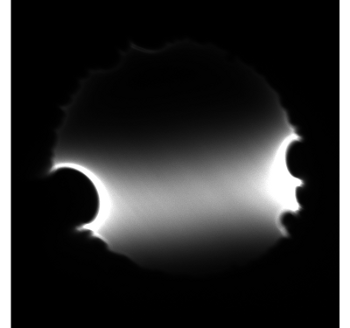
\includegraphics{final-fourier-030.png}};
  \draw [very thick,red] (6,-0.4) -- ++(9:2.2);

  \draw [thick,->,green] 
    (0,-3.5) -- ++(3,0) 
      node [pos=0.5,below,black,align=center] {$k_L \sin \theta$\\$\theta \approx 47^{\circ}$}
  ;
  \draw [thick,dashed,green] 
    (3,-3.5) -- (4,-3.5)
      node [above,black,pos=0.8] {$45^{\circ}$}
  ;
  \draw [thick,->,red]
    (3,-3.5) -- ++(1.4,1.4)
      node [pos=0.4,left,black] {$k_G$}
      coordinate [pos=1] (end)
  ;
  \draw [thick,->,blue]
    (0,-3.5) -- (end)
      node [pos=0.5,black,above] {$k_{SP}$}
  ;
  \node at (7,-3) {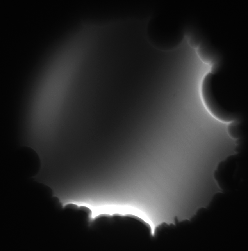
\includegraphics{rotated.png}};
  \draw [very thick,green,dashed] 
    (6,-2.7) -- ++(9:2.2)
      node [pos=0.7,below, white] {$45^{\circ}$}
      coordinate [pos=1] (rotate end)
  ;
  \draw [very thick,red]
    (rotate end) -- ++(234:2.2)
  ;
\end{tikzpicture}
